%!TEX root = paper.tex
\chapter{A tour of \Backpack{}}
\label{sec:tour}

In this section, we give a ``user's eye'' tour of the extensions to
Cabal and GHC which constitute \Backpack{}.  While \Backpack{} is in
many respects similar to \OldBackpack{}~\cite{backpack}, we will not assume
familiarity with Backpack or Cabal; however, we will pay close attention
to aspects of the design which facilitate the split of \Backpack{}
across the package manager and compiler.

\section{The current state of affairs}

A \emph{package} is the unit of distribution, versioning, and sharing,
and a \emph{package manager} allows developers to reuse code
written by other people.  In the case of Haskell, Cabal is the package manager for GHC
and Hackage is the site where Cabal packages are uploaded and indexed.
Each Cabal package has a \emph{Cabal file}, which describes
one or more \emph{components} (libraries, executables, test-suites, etc.), each of which
defines modules (with source code in separate files, ommitted from our examples) and specifies dependencies on other packages.  Here are four
example Cabal files, each describing a single component\footnote{
Though a package is not synonymous with a component, they are
often conflated, since in Cabal, a dependency on a package actually
specifies a dependency on the library component of the package.}:

\begin{verbatim}
  name: base
  library
    exposed-modules: Prelude

  name: bytestring
  library
    build-depends: base
    exposed-modules: Data.ByteString

  name: mysql
  library
    build-depends: base, bytestring
    exposed-modules: Db.MySQL

  name: mysql-dsl
  library
    build-depends: base, mysql, bytestring
    exposed-modules: DSL.MySQL
\end{verbatim}
%
% We omit the separate Haskell source files for each of the modules defined
% in these packages.
Given a package description, Cabal automates the process of retrieving
its dependencies, determining a build order, interfacing with
GHC to build them and installing the results.\footnote{Strictly speaking,
Cabal handles the process of building a single package, while
cabal-install handles the process of building multiple packages.  In
practice, however, there is a lot of overlap between the functionality the two
implement, so we refer to both as Cabal in this paper.}

\paragraph{Status quo ``modularity'' via versions}
A \verb|build-depends| field also specifies acceptable
version range for a dependency:

\begin{verbatim}
  name: mysql
  version: 1.0
  library
    build-depends: base, bytestring >= 0.9
    exposed-modules: Db.MySQL

  name: mysql-dsl
  version: 1.0
  library
    build-depends:
      base, mysql == 1.*, bytestring >= 0.10
    exposed-modules: DSL.MySQL
\end{verbatim}
Thus, a \verb|build-depends| constraint is not a completely definite
reference: the specific version of a dependency is chosen by Cabal's
\emph{dependency resolution} step, allowing libraries to be reused at different
versions of their dependencies.

\begin{figure}
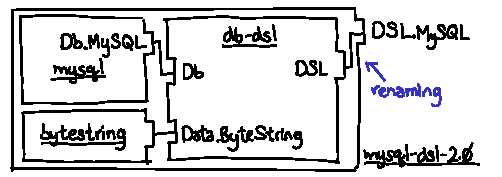
\includegraphics{diagrams/programming-against-interface.pdf}
\caption{\emph{Programming against an interface.} This is the wiring
diagram for \texttt{mysql-dsl-2.0}.  The left side of the blocks
(representing components) have input ports (required signatures),
while the right hand side have output ports (provided modules).  Ports are wired up to show how
requirements are filled; a kink indicates that some renaming took place.
Mixin linking wires up requirements and provisions which have the same
module name.}
\label{fig:programming-against-interface}
\end{figure}

\section{Programming against an interface}

The \verb|build-depends|
constraints have the limitation of committing to a specific
library (albeit not a specific version) to implement a dependency.  Perhaps this is fine for
\verb|base|, but we may not want to force \verb|mysql| on the users of \verb|mysql-dsl|
---they should be able to use our library with any database that
implements the required interface.
In \Backpack{}, a direct dependency can be replaced with a
\emph{required signature}:

\begin{verbatim}
  name: db-dsl
  library
    build-depends: base
    required-signatures: Data.ByteString, Db
    exposed-modules: DSL
\end{verbatim}
Two new files, \verb|Db.hsig| and \verb|Data/ByteString.hsig|, accompany the package description and give
the signatures of the functions used by \verb|db-dsl|.
A library with requirements is \emph{uninstantiated}: it can be typechecked but not
run.  Every signature source file specifies the types, instances, functions, values, etc., which must be provided
by any module implementing this requirement.  For example, the source for
\verb|Db.hsig| might be:

\begin{verbatim}
  signature Db where
    import Prelude (IO)
    import Data.ByteString (ByteString) -- a sig!
    data Connection
    run :: Connection -> ByteString -> IO ()
\end{verbatim}
%
A client can instantiate a requirement merely by having a module
in scope with the same module name as the requirement; a process called \emph{mixin linking} instantiates the requirement.  Below, we instantiate \verb|db-dsl| with \verb|mysql| and
\verb|bytestring| (depicted in Figure~\ref{fig:programming-against-interface}):

\begin{verbatim}
  name: mysql-dsl
  version: 2.0
  library
    build-depends: db-dsl, mysql, bytestring
    backpack-includes: mysql (Db.MySQL as Db)
    reexported-modules: DSL as DSL.MySQL
\end{verbatim}
%
\verb|db-dsl|'s requirements \verb|Data.ByteString| and \verb|Db| are
filled by the modules provided by packages \verb|bytestring| and \verb|mysql|,
respectively.  Note that in the case of \verb|mysql|, the module has the wrong
name, so we use the \verb|backpack-includes|\footnote{Cabal already uses
\texttt{includes} to denote C header includes.} to rename it to the correct name.
Additionally, the \verb|reexported-modules| line
reexports \verb|db-dsl|'s module under a new name \verb|DSL.MySQL|.

A practical consideration is whether or not there is any performance
cost to using signatures.  In particular, if one separately compiles
uninstantiated components to machine code, no cross-package inlining
can occur, since the component is compiled only against a signature
and not against the code that implements the signature.
For Haskell and GHC, cross-module inlining is a major contributor to performance,
so \Backpack{} does \emph{not}
separately compile uninstantiated packages. Instead, every distinct
instantiation of a component is compiled against the code that implements
its requirements. This process is managed by
Cabal to avoid unnecessary recompilation, similarly to how Cabal
avoids recompiling dependencies that are already installed.

\section{Reusing libraries with different instantiations}

\begin{figure}
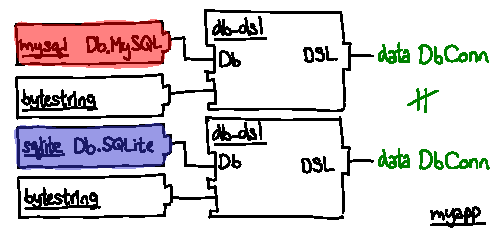
\includegraphics{diagrams/reusing-packages-functors.pdf}
\caption{\emph{Reusing libraries like functors.}  Here, we consider
two instantiations of \texttt{db-dsl} which define \texttt{data DbConn}.
The two \texttt{DbConn}s are not type equivalent, because the respective
wiring diagrams they are associated with are not equal.}
\label{fig:reusing-packages-functors}
\end{figure}

Suppose an application wants to use \verb|db-dsl| with two different databases
at the same time. It can do so by mentioning \verb|db-dsl| twice in
\verb|backpack-includes| (depicted in Figure~\ref{fig:reusing-packages-functors}):

\begin{verbatim}
  name: myapp
  library
    build-depends:
      db-dsl, mysql, sqlite, bytestring
    backpack-includes:
      db-dsl (DSL as DSL.MySQL)
        requires (Db as Db.MySQL)
      db-dsl (DSL as DSL.SQLite)
        requires (Db as Db.SQLite)
    exposed-modules: App
\end{verbatim}
%
This gives us two copies of \verb|db-dsl|: one with \verb|Db| filled
with \verb|Db.MySQL|, and one with \verb|Db| filled with
\verb|Db.SQLite|.

However, an important subtlety arises in
this situation.  Ordinarily, two types are considered equivalent if they
have the same \emph{identity}: an identity consists of both the name of the
type and the name of the module which originally defined the type.
Suppose, however, that \verb|db-dsl| contained a module which defined
a type:

\begin{verbatim}
  module DSL(DbConn) where
    import Db
    data DbConn = DbConn Connection URL
\end{verbatim}
%
The identity of \verb|DbConn| must somehow depend on how
we decided to implement \verb|Connection|: the \verb|DbConn| backed by
\verb|mysql| is distinct from the \verb|DbConn| backed by \verb|sqlite|
(after all, they may contain utterly different \verb|Connection| values).
Thus, in \Backpack{}, the identity of a type
also contains the \emph{wiring} diagrams of the components which
defined the types in question.  Now, the two \verb|DbConn|s come from
distinct \verb|db-dsl|s which have different wiring diagrams;
thus, they are distinct types in Haskell.

\section{Composing libraries with requirements}

\begin{figure}
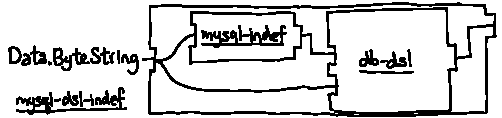
\includegraphics{diagrams/composing-requirements.pdf}
\caption{\emph{Composing libraries with requirements.} It is possible
to use components without filling all of their requirements; in that
case, those requirements are propagated to the requirements of the
enclosing component.}
\label{fig:composing-requirements}
\end{figure}

Unlike functors, it is easy to use mixin linking to only partially
instantiate components or combine their requirements.  For example,
consider this alternate version of \verb|mysql| with a requirement:

\begin{verbatim}
  name: mysql-indef
  library
    build-depends: base
    required-signatures: Data.ByteString
    exposed-modules: Db.MySQL
\end{verbatim}
%
One might like to reformulate \verb|mysql| like this so that it can
be used with any package implemeting the \verb|Data.ByteString| interface.
We can use this package to create a version of \verb|db-dsl|
which is partially instantiated: that is, it is instantiated
with \verb|mysql-indef|, but leaves \verb|Data.ByteString|
unimplemented (depicted in Figure~\ref{fig:composing-requirements}):

\begin{verbatim}
  name: mysql-dsl-indef
  library
    build-depends: db-dsl, mysql-indef
    backpack-includes: mysql-indef (Db.MySQL as Db)
    reexported-modules: DSL.Db as DSL.Db.MySQL
\end{verbatim}
%
\verb|mysql-dsl-indef| has an implicit requirement
\verb|Data.ByteString|, which is the \emph{merge} of the
requirements of \verb|db-dsl| and \verb|mysql-indef|.  For
example, if we have the requirements:

\begin{verbatim}
  -- db-dsl's requirement
  signature Data.ByteString
    data ByteString
    length :: ByteString -> Int

  -- mysql-indef's requirement
  signature Data.ByteString
    data ByteString
    concat :: [ByteString] -> ByteString
\end{verbatim}
%
The merged requirement is:

\begin{verbatim}
  signature Data.ByteString
    data ByteString
    length :: ByteString -> Int
    concat :: [ByteString] -> ByteString
\end{verbatim}
%
Notice that the two type declarations for \verb|ByteString| have been
merged to one: this is how mixin linking eliminates the need
for sharing constraints!

%%% Local Variables:
%%% mode: latex
%%% TeX-master: "paper"
%%% End:
